\subsection{Caminhada do gato}

\begin{questions}
\question{
A Figura \ref{fig:catwalk} apresenta a planta de uma casa.
Algumas portas da casa são de duplo-sentido, enquanto outras possuem
sentido único, o que pode ser verificado na representação através das setas.
Um gato caminha aleatoriamente pela casa. Quando o gato está em um cômodo,
ele pode permanecer neste cômodo ou utilizar alguma porta para trocar de cômodo.
Suponha que, a cada instante, o gato escolha entre as alternativas com igual probabilidade.
Como existe um cachorro no quarto 3, o gato não permanece neste quarto, deixando-o
imediatamente no próximo instante após ingressar neste quarto.
\begin{figure}[!ht]
\centering
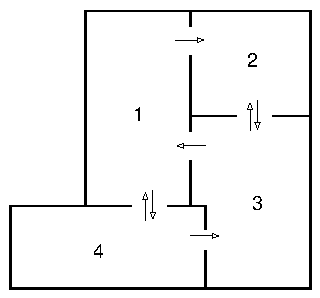
\includegraphics[width=0.3\textwidth]{../images/catwalk.pdf}
\caption{Caminhada do gato em uma casa.}
\label{fig:catwalk}
\end{figure}

\begin{parts}
\part Encontre a matriz de transição e a cadeia de Markov para este problema (desenhe o grafo).

\part Qual é a distribuição em estado estacionário para o quarto no qual o gato está?
%\textit{(dica: utilize a equação que representa a condição de estacionariedade;
%leve todos os termos para um lado da equação, para obter uma igualdade com zero;
%coloque em evicência; para adicionar a condição $\sum_i \mu_i = 1$, troque a
%última coluna da matriz por uma coluna com uns e troque o último zero do vetor por um;
%resolva o sistema)} 

\part Calcule a taxa de entropia para a caminhada do gato.
\end{parts}
}

\begin{solution}
\begin{parts}
\part 
Poderemos considerar os quartos como estados em uma cadeia de Markov. Desta forma, 
a matriz de transição é dada por
\begin{equation}
P = \begin{pmatrix} 
\frac{1}{3} & \frac{1}{3} & 0 & \frac{1}{3} \\
0 & \frac{1}{2} & \frac{1}{2} & 0 \\
\frac{1}{2} & \frac{1}{2} & 0 & 0 \\
\frac{1}{3} & 0 & \frac{1}{3} & \frac{1}{3} 
\end{pmatrix} .
\end{equation}

A cadeia de Markov é ilustrada a seguir:
\begin{center}
\begin{tikzpicture}[->, >=stealth', auto, semithick, node distance=3cm]
\tikzstyle{every state}=[fill=white,draw=black,thick,text=black,scale=1]
\node[state]    (1)               {$1$};
\node[state]    (2)[right of=1]   {$2$};
\node[state]    (4)[below of=1]   {$4$};
\node[state]    (3)[below of=2]   {$3$};
\path
(1) edge[loop left]        node{$1/3$}  (1)
(1) edge[bend left,above]  node{$1/3$}  (2)
(1) edge[bend left, right]  node{$1/3$}  (4)
(2) edge[loop right]       node{$1/2$}  (2)
(2) edge[bend left,right]  node{$1/2$}  (3)
(3) edge[bend left,left]   node{$1/2$}  (2)
(3) edge[above]      node{$1/2$}  (1)
(4) edge[loop below]       node{$1/3$}  (4)
(4) edge[bend left, left]  node{$1/3$}  (1)
(4) edge[bend right, below] node{$1/3$}  (3)
;
\end{tikzpicture}
\end{center}


\part 
A distribuição de estado estacionário é tal que $\mathbf{\mu}^T P = \mathbf{\mu}^T$, com $\sum_i \mu_i = 1$.

\begin{eqnarray}
\mathbf{\mu}^T P &=& \mathbf{\mu}^T \\
\mathbf{\mu}^T (P-I) &=& 0 \\
\mathbf{\mu}^T Q &=& 0 
\end{eqnarray}
Teremos aqui 
\begin{equation}
Q = \begin{pmatrix} 
-\frac{2}{3} & \frac{1}{3} & 0 & \frac{1}{3} \\
0 & -\frac{1}{2} & \frac{1}{2} & 0 \\
\frac{1}{2} & \frac{1}{2} & -1 & 0 \\
\frac{1}{3} & 0 & \frac{1}{3} & -\frac{2}{3} 
\end{pmatrix} .
\end{equation}

Note que, no sistema de equações acima, podemos incorporar a condição $\sum_i \mu_i = 1$ bastando
para tanto substituir uma das colunas da matriz $Q$ por uma coluna com uns e substituir
um dos zeros no vetor de zeros do lado direito da equação por um na posição respectiva.
Podemos, por exemplo, escolher a última coluna de $Q$ e assim teremos uma matriz 
\begin{equation}
\tilde{Q} =
\begin{pmatrix} 
-\frac{2}{3} & \frac{1}{3} & 0 & 1 \\
0 & -\frac{1}{2} & \frac{1}{2} & 1 \\
\frac{1}{2} & \frac{1}{2} & -1 & 1 \\
\frac{1}{3} & 0 & \frac{1}{3} & 1
\end{pmatrix} ,
\end{equation}
e o novo sistema de equações será
\begin{equation}
\mathbf{\mu}^T \tilde{Q} = (0, 0, 0, 1) ,
\end{equation}
e a solução poderá ser obtida pós-multiplicando pela matriz inversa de $\tilde{Q}$,
\begin{equation}
\mathbf{\mu}^T = (0, 0, 0, 1) \tilde{Q}^{-1} .
\end{equation}

Calculando a inversa, encontramos
\begin{equation}
\tilde{Q}^{-1} =
\begin{pmatrix} 
-\frac{21}{25} & -\frac{2}{5} & \frac{4}{25} & \frac{27}{25} \\
\frac{3}{5} & -2 & -\frac{2}{5} & \frac{9}{5} \\
\frac{3}{25} & -\frac{4}{5} & -\frac{22}{25} & \frac{39}{25} \\
\frac{6}{25} & \frac{2}{5} & \frac{6}{25} & \frac{3}{25}
\end{pmatrix} ,
\end{equation}
e assim,
\begin{equation}
\mathbf{\mu}^T = (\frac{6}{25}, \frac{2}{5}, \frac{6}{25}, \frac{3}{25}) .
\end{equation}

Para resolver o sistema, faremos
\begin{eqnarray}
\mathbf{\mu}^T \tilde{Q} &=& \begin{pmatrix} 0 & 0 & 0 & 1  \end{pmatrix} \\
\left( \mathbf{\mu}^T \tilde{Q} \right)^T &=& \begin{pmatrix} 0 & 0 & 0 & 1  \end{pmatrix}^T \\
\tilde{Q}^T \mathbf{\mu}  &=& \begin{pmatrix} 0 \\ 0 \\ 0 \\ 1  \end{pmatrix} .
\end{eqnarray}

Iremos aplicar as operações elementares à matriz $\tilde{Q}^T$ aumentada para solucionar o sistema:
\begin{equation}
\begin{blockarray}{cccccc}
\begin{block}{c(cccc|c)}
 l_1 & -2/3 & 0    & 1/2 & 1/3 & 0  \\
 l_2 & 1/3  & -1/2 & 1/2 & 0   & 0  \\
 l_3 & 0    & 1/2  & -1  & 1/3 & 0  \\
 l_4 & 1    & 1    & 1   & 1   & 1  \\
\end{block}
\end{blockarray} 
\end{equation}


\begin{equation}
\begin{blockarray}{cccccc}
\begin{block}{c(cccc|c)}
 -\frac{3}{2} l_1      & 1    & 0    & -3/4 & -1/2 & 0  \\
 l_2 + \frac{1}{2} l_1 & 0    & -1/2 & 3/4  & 1/6  & 0  \\
 2 l_3                 & 0    & 1    & -2   & 2/3  & 0  \\
 l_4 + \frac{3}{2} l_1 & 0    & 1    & 7/4  & 3/2  & 1  \\
\end{block}
\end{blockarray} 
\end{equation}

\begin{equation}
\begin{blockarray}{cccccc}
\begin{block}{c(cccc|c)}
 l_1         & 1    & 0    & -3/4 & -1/2 & 0  \\
 -2 l_2      & 0    & 1    & -3/2 & -1/3 & 0  \\
 l_3 + 2 l_2 & 0    & 0    & -1/2 & 1    & 0  \\
 l_4 + 2 l_2 & 0    & 0    & 13/4 & 11/6 & 1  \\
\end{block}
\end{blockarray} 
\end{equation}

\begin{equation}
\begin{blockarray}{cccccc}
\begin{block}{c(cccc|c)}
 l_1                    & 1    & 0    & -3/4 & -1/2 & 0  \\
 l_2                    & 0    & 1    & -3/2 & -1/3 & 0  \\
 -2 l_3                 & 0    & 0    & 1    & -2   & 0  \\
 l_4 + \frac{13}{2} l_3 & 0    & 0    & 0    & 25/3 & 1  \\
\end{block}
\end{blockarray} 
\end{equation}

Podemos assim concluir que:
\begin{eqnarray}
\mu_4 &=& \frac{3}{25} \\
\mu_3 &=& 2 \mu_4 = \frac{6}{25} \\
\mu_2 &=& \frac{3}{2} \mu_3 + \frac{1}{3} \mu_4 = \frac{2}{5} \\
\mu_1 &=& \frac{3}{4} \mu_3 + \frac{1}{2} \mu_4 = \frac{6}{25} .
\end{eqnarray}

e assim
\begin{equation}
\mathbf{\mu}^T = (\frac{6}{25}, \frac{2}{5}, \frac{6}{25}, \frac{3}{25}) .
\end{equation}


\part
A taxa de entropia para um cadeia de Markov de primeira ordem estacionária será dada da seguinte forma
\begin{eqnarray}
  H(\mathcal{X}) &=&  \sum_i \mu_i \left[ - \sum_j p_{ij} \log p_{ij} \right] \\
        &=& \sum_i \mu_i H(\mathbf{p}_i^T) \\
        &=& \frac{6}{25} H\left(\frac{1}{3}, \frac{1}{3}, 0, \frac{1}{3} \right) +
        \frac{2}{5} H\left(0, \frac{1}{2}, \frac{1}{2}, 0 \right) +
        \frac{6}{25} H\left(\frac{1}{2}, \frac{1}{2}, 0, 0 \right) + 
        \frac{3}{25} H\left(\frac{1}{3}, 0, \frac{1}{3}, \frac{1}{3} \right) \\
        &=& \frac{6}{25} \log 3 + \frac{2}{5} + \frac{6}{25} + \frac{3}{25} \log 3 \\
        &=& \frac{9}{25} \log 3 + \frac{16}{25} \approx 1.2106
\end{eqnarray}


\end{parts}
\end{solution}
\end{questions}
